Tato kapitola se zabývá porovnáním jednotlivých technik pro detekci a~klasifikaci značek popsaných v~kapitolách \ref{detekceZnacek} a~\ref{detekceKonv}, návrhem systému pro detekci dopravního značení, a~také porovnáním datových sad a~neuronových sítí, které lze použít k~trénování a~testování.

%%%%%%%%%%%%%%%%%%%%%%%%%%%%%%%%%%%%%%%%%%%%%%%%%%%%%%%%%%%%%%%%%%%%%%%%%%%%%%%%%%%%%%%%%%%

\section{Datové sady dopravního značení}
\label{datoveSady}
Datové sady jsou neodmyslitelnou součástí strojového učení. Dostatek datových sad je jedním z~důvodů, proč se neuronové sítě staly v~dnešní době tak populárními. Datových sad dopravních značek existuje spousta, avšak většina z~nich obsahuje pouze vyřezané dopravní značky z~celých snímků, na kterých se běžně trénují klasifikátory (tedy systémy, které slouží pouze k~rozhodnutí o~třídě značky, nikoli k~detekci a~lokalizaci v~rámci celého snímku). Běžná velikost snímků v~takovýchto sadách bývá velmi malá, například $64 \times 64$ pixelů. Jak je popsáno v~sekci \ref{yoloTeorie}, systém YOLO použitý v~této práci pro detekci se trénuje na tzv. celých (nebo také plných) snímcích. Dokáže se z~nich naučit jak celkový kontext, tak i~relativní velikost detekovaných značek. Proto bylo potřeba najít takovou datovou sadu, která bude obsahovat celé snímky.

Podařilo se najít čtyři takové datové sady dopravních značek: Německou (GTSD) \cite{gtsd}, Belgickou (BTSD) \cite{btsd}, Ruskou (RTSD) \cite{rtsd} a~Americkou, kde však používají naprosto rozdílnou normu dopravního značení, a~proto byla v~rámci této práce nepoužitelná. Počáteční písmeno těchto datových sad běžně slouží k~jejich identifikaci (název státu, kde byly snímky pořízeny) a~končí písmenem ``D'', které je zkratkou pro anglické \emph{detection} a~běžně značí, že se jedná o~datovou sadu s~celými snímky používanými pro detekci. Stejně tak ``C'' jako \emph{classification}. V~tabulce \ref{tabulkaDatasety} lze najít velikost jednotlivých sad, dále pak počet tříd a~značek v~nich obsažených.

\begin{table}[H]
	\vskip6pt
	\centering
    \begin{tabular}{ l | c | c | c }
        Datová sada & Počet snímků & Počet tříd & Počet značek \\
        \toprule
        GTSD \cite{gtsd} & 900 & 43 & 1213 \\
        BTSD \cite{btsd} & 25630 & 108 & 13444 \\
        RTSD \cite{rtsd} & 179138 & 156 & 104358 \\
    \end{tabular}
    \caption{Tabulka velikostí, počtu tříd a~značek jednotlivých datových sad značek.}
    \vskip6pt
    \label{tabulkaDatasety}
\end{table}

Na obrázku \ref{fig:datasety} lze vidět ukázku snímků z~jednotlivých datových sad. Jak lze vidět v~tabulce \ref{tabulkaDatasety}, velikost jednotlivých datových sad se liší. Stejně tak se liší kvalita, velikosti a~anotace snímků.

\begin{figure}[H]
    \centering
    \tmpframe{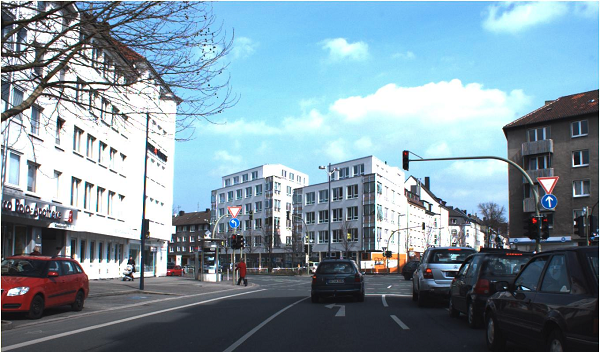
\includegraphics[width=0.33\linewidth]{figures/datasety/gtsd.png}}\hfill
    \tmpframe{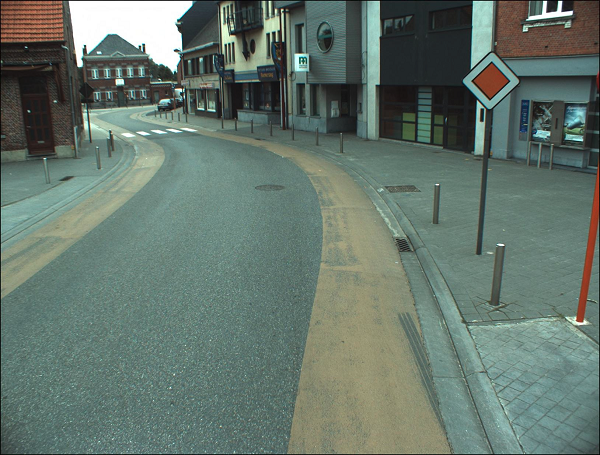
\includegraphics[width=0.33\linewidth]{figures/datasety/btsd.png}}\hfill
    \tmpframe{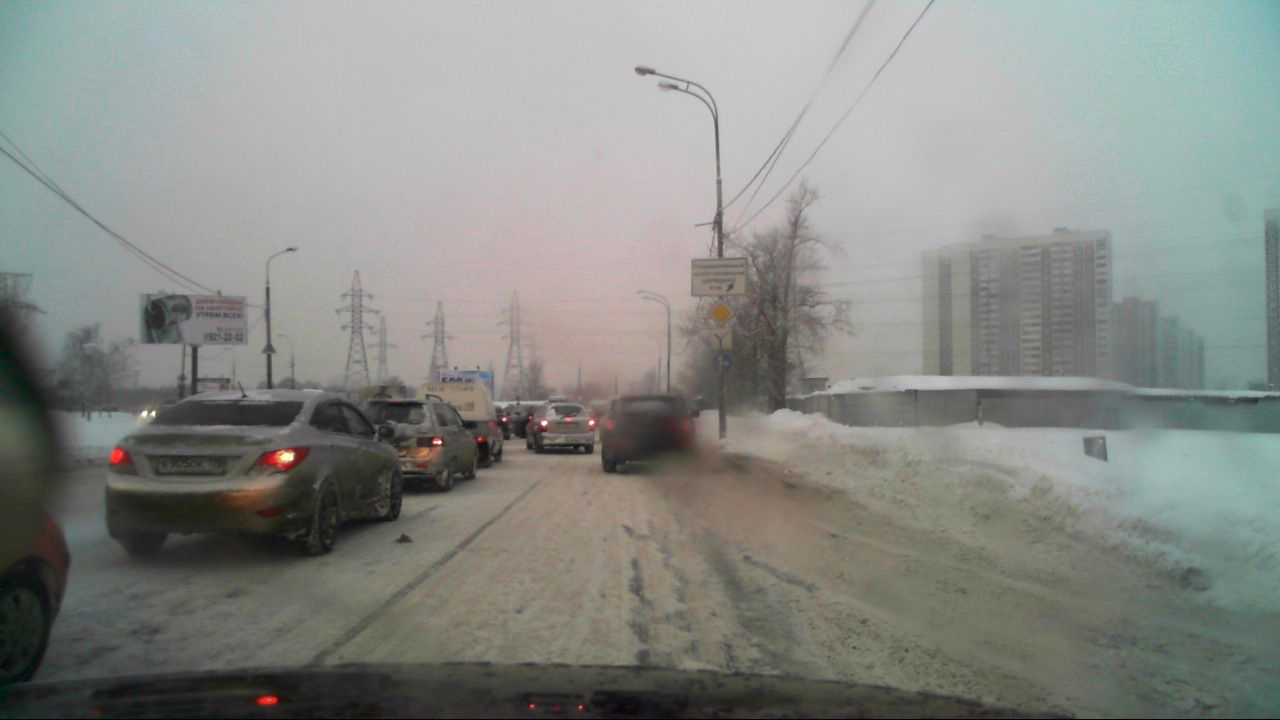
\includegraphics[width=0.33\linewidth]{figures/datasety/rtsd.png}}
    \caption{Ukázka snímků datových sad (\textbf{zleva}) GTSD, BTSD a~RTSD.}
    \label{fig:datasety}
\end{figure}

Nejvyšší kvalitu má Německá datová sada, tedy GTSD, avšak nevýhoda této sady je velmi malý počet značek na třídu -- v~průměru to je cca. 28, a~to pro natrénování a zároveň vyhodnocení kvalitního detektoru nestačí. Ruská datová sada má naopak značek na třídu dost, ale kvalita těchto značek a~snímků obecně je velmi špatná. Značky jsou malé a~rozmazané. Jako dostatečná se tedy jeví Belgická sada, která má poměrně dost snímků i~dobrou kvalitu, ale nevýhodou této sady je, že téměř dvě třetiny datové sady je pouze tzv. \emph{negativní datová sada} (neobsahující žádné značky). I přes to ale byla tato sada vybrána jako hlavní pro trénování i testování.


%%%%%%%%%%%%%%%%%%%%%%%%%%%%%%%%%%%%%%%%%%%%%%%%%%%%%%%%%%%%%%%%%%%%%%%%%%%%%%%%%%%%%%%%%%%


\section{Návrh generátoru syntetických dat}
Z~důvodu nedostatku datových sad dopravních značek s~plnými snímky, a~také za účelem porovnání detektoru trénovaného na reálných a~syntetických datech jsem se rozhodl v~rámci této práce vytvořit generátor syntetických datových sad. Cílem bylo iterativně zlepšovat generátor, aby výsledná data co nejvíce odpovídala reálným snímkům a~zlepšování výsledků, aby se kvalita detektoru trénovaného na syntetických datech vyrovnala, či dokonce překonala kvalitu detektoru trénovaného na reálných datech. Testování obou detektorů probíhalo na reálných snímcích Belgické sady. Aby se syntetická data co nejvíce podobala reálným snímkům, je potřeba dosáhnout velké variability snímků simulující různé světelné podmínky, přírodní vlivy, natočení, vandalismus, apod. To následně umožňuje hluboké konvoluční síti se naučit dostatek vlastností a~dokázat správně generalizovat na reálných snímcích. Z důvodu, že se zvolená metoda YOLO učí i~celkový kontext ve kterém se objekty nachází, byly pro generování využity jako pozadí snímky zachycené z~jedoucího vozidla (převážně v~městské zástavbě), neobsahující žádné značky. Značky, které by nebyly anotovány a negativně by ovlivňovaly proces trénování.

Alternativním způsobem pro získání kvalitní dostatečně velké anotované datové sady, bez nutnosti anotace každého snímku jednotlivě, by bylo využití existujícího detektoru značek (pokud možno toho s~nejvyšší úspěšností) a~jeho aplikování na ne-anotovanou datovou sadu. Poté by stačilo výsledky projít a~případně upravit nevalidní detekce, což by zabralo podstatně méně času, než anotovat celou datovou sadu ručně. Protože částečným cílem práce je i~porovnání modelů trénovaných na reálných a~syntetických datech, rozhodl jsem se tento způsob nevyužít a~soustředit se na tvorbu syntetické datové sady.


%%%%%%%%%%%%%%%%%%%%%%%%%%%%%%%%%%%%%%%%%%%%%%%%%%%%%%%%%%%%%%%%%%%%%%%%%%%%%%%%%%%%%%%%%%%


\section{Porovnání a~výběr metod pro detekci a~klasifikaci}
\label{navrhDetekce}
Tato práce si dává za cíl použití \textbf{moderních technik pro detekci}, a~proto se do užšího výběru dostaly pouze metody jako SSD, YOLO, Fast(er) R-CNN a~RetinaNet. V~tabulce~\ref{tab:porovnaniMetody} lze vidět komplexní porovnání úspěšností těchto metod na datové sadě COCO. Tabulka zobrazuje úspěšnost AP v~závislosti na různých prazích IoU a~různých velikostech detekovaných objektů (\emph{small}, \emph{medium} a~\emph{large}, tzn. malé, střední a velké). Tabulka je rozdělena na dvě části podle počtu kroků vykonávaných systémem při detekci. Protože při detekci je důležitá také rychlost, je na obrázku \ref{fig:porovnaniDetektoru} graficky znázorněno porovnání metod podle času potřebného pro vyhodnocení jednoho snímku v~závislosti na úspěšnosti.

\begin{table}[H]
	\vskip6pt
	\centering
    \begin{tabular}{ l | c | c c c | c c c }
        & Backbone & AP & AP_{50} & AP_{75} & AP_S & AP_M & AP_L \\
        \toprule
        \emph{Two-stage methods} & & & & & & & &
        Faster R-CNN+++ & ResNet-101-C4 & 34.9 & 55.7 & 37.4 & 15.6 & 38.7 & 50.9 \\
        Faster R-CNN & ResNet-101-FPN & 36.2 & 59.1 & 39.0 & 18.2 & 39.0 & 48.2 \\
        w FPN & & & & & & & \\
        Faster R-CNN & Inception-ResNet-v2 & 34.7 & 55.5 & 36.7 & 13.5 & 38.1 & 52.0 \\
        by G-RMI & & & & & & & \\
        Faster R-CNN & Inception-ResNet-v2 & 36.8 & 57.7 & 39.2 & 16.2 & 39.8 & \textbf{52.1} \\
        w TDM & TDM & & & & & & \\
        \hline
        \emph{One-stage methods} & & & & & & & &
        YOLOv2 & DarkNet-19 & 21.6 & 44.0 & 19.2 & 5.0 & 22.4 & 35.5 \\
        SSD513 & ResNet-101-SSD & 31.2 & 50.4 & 33.3 & 10.2 & 34.5 & 49.8 \\
        DSSD513 & ResNet-101-DSSD & 33.2 & 53.3 & 35.2 & 13.0 & 35.4 & 51.1 \\
        RetinaNet & ResNet-101-FPN & 39.1 & 59.1 & 42.3 & 21.8 & 42.7 & 50.2 \\
        RetinaNet & ResNeXt-101-FPN & \textbf{40.8} & \textbf{61.1} & \textbf{44.1} & \textbf{24.1} & \textbf{44.2} & 51.2 \\
        YOLOv3 $608 \times 608$ & Darknet-53 & 33.0 & 57.9 & 34.4 & 18.3 & 35.4 & 41.9 \\
    \end{tabular}
    \caption{Porovnání detekčních metod na různých metrikách~\cite{yolov3}.} 
    \vskip6pt
    \label{tab:porovnaniMetody}
\end{table}

Jak lze z~tabulky vyčíst, rozdíl mezi SSD a~YOLOv3 v~rámci úspěšnosti při použití moderní metriky AP, počítané na 10 různých prazích IoU, není velký a~oba tyto systémy předčil model RetinaNet. Při použití tradiční metriky $AP_{50}$, počítané pouze na $\text{IoU} = 0.5$ má YOLOv3 velmi dobrou úspěšnost srovnatelnou s~RetinaNet a~podstatně lepší úspěšnost než obě verze SSD. Se zvyšujícím se prahem IoU značně klesá úspěšnost metod YOLOv3 a~SSD, což indikuje nedokonalou lokalizaci objektů (predikované boxy neodpovídají přesně \emph{ground-truth}, tedy skutečné pozici objektů).

Protože u~SSD slouží k~detekci pouze několik počátečních vrstev, je úspěšnost detekce malých objektů poměrně nízká. V~minulosti mělo s~detekcí malých objektů velké problémy i~YOLO, ale třetí verze provádějící detekci na třech různých rozlišeních značně zlepšila jejich detekci, ale stále je podstatně nižší než u~RetinaNet.

\begin{figure}[H]
    \centering
    \tmpframe{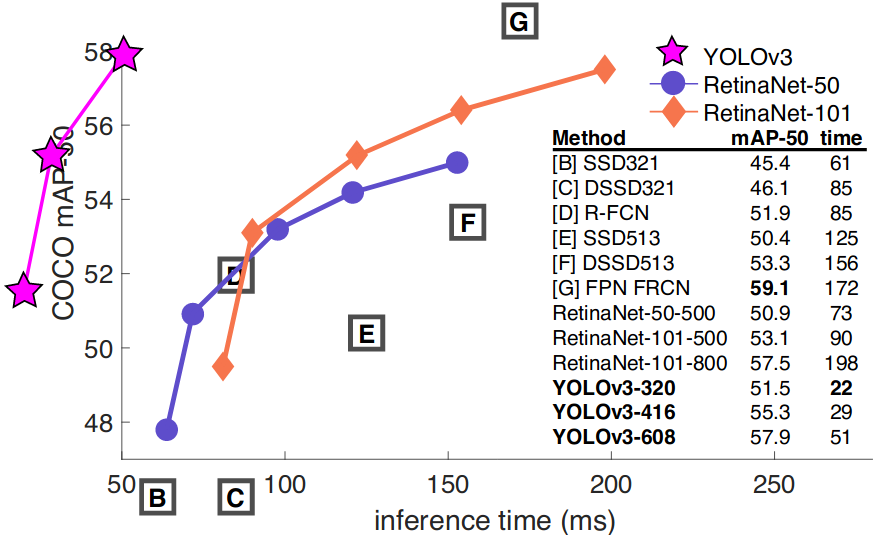
\includegraphics[width=0.85\linewidth]{figures/navrh/porovnaniDetektoru.png}}
    \caption{Porovnání detekčních systémů v~poměru úspěšnosti a~rychlosti vyhodnocení detekce na GPU Titan X.\footnotemark}
    \label{fig:porovnaniDetektoru}
\end{figure}

\footnotetext{Převzato z~\cite{yolov3}.}

YOLOv3 je jednoznačně nejrychlejší metodou ze všech uvedených a~i~přesto dosahuje velmi dobré úspěšnosti detekce. Odlehčená verze dokonce dosahuje dokonce rychlosti až 150 snímků za sekundu výměnou za několik bodů mAP. Při použití běžné grafické karty (oproti Titan X, na níž jsou uvedené rychlosti získány) výrazně klesne rychlost trénování a~zejména detekce, a~proto jsem se rozhodl použít systém Tiny YOLOv3, což je již zmíněná odlehčená verze systému YOLOv3, se kterou by bylo možné dosáhnout zpracování v~reálném čase i~na běžné grafické kartě a~přitom dosáhnout dobré úspěšnosti detekce.


%%%%%%%%%%%%%%%%%%%%%%%%%%%%%%%%%%%%%%%%%%%%%%%%%%%%%%%%%%%%%%%%%%%%%%%%%%%%%%%%%%%%%%%%%%%


\section{Neuronová síť Darknet}
\label{navrhDarknet}
Darknet \cite{darknet} je \emph{open-source} (česky otevřený software) aplikační rámec neuronové sítě napsané v~programovacím jazyce \texttt{C} a~\texttt{CUDA}\footnotemark. Je možné s~ním provádět výpočty jak na CPU (procesoru), tak na GPU (grafické kartě). \emph{Darknet} je možné používat jak na operačním systému Linux, tak i~upravenou verzi na systému Windows.

\begin{table}[H]
	\vskip6pt
	\centering
    \begin{tabular}{ l | c c c c c }
        Backbone & Top-1 & Top-5 & Bn Ops & BFLOPS/s & FPS \\
        \toprule
        Darknet-19 & 74.1 & 91.8 & 7.29 & 1246 & \textbf{171} \\
        ResNet-101 & 77.1 & 93.7 & 19.7 & 1039 & 53 \\
        ResNet-152 & \textbf{77.6} & \textbf{93.8} & 29.4 & 1090 & 37 \\
        Darknet-53 & 77.2 & \textbf{93.8} & 18.7 & \textbf{1457} & 78 \\
    \end{tabular}
    \caption{Porovnání neuronových sítí: Přesnost, počet bilionů operací bez i~s~plovoucí řádovou čárkou a~počet snímků za sekundu~\cite{yolov3}.} 
    \vskip6pt
    \label{tab:porovnaniBackbones}
\end{table}

 Kvůli parametrům neuronové sítě Darknet-53 jsem se rozhodl ji použít v této práci.

\footnotetext{CUDA -- \emph{Compute Unified Device Architecture}.}